% The document class supplies options to control rendering of some standard
% features in the result.  The goal is for uniform style, so some attention 
% to detail is *vital* with all fields.  Each field (i.e., text inside the
% curly braces below, so the MEng text inside {MEng} for instance) should 
% take into account the following:
%
% - author name       should be formatted as "FirstName LastName"
%   (not "Initial LastName" for example),
% - supervisor name   should be formatted as "Title FirstName LastName"
%   (where Title is "Dr." or "Prof." for example),
% - degree programme  should be "BSc", "MEng", "MSci", "MSc" or "PhD",
% - dissertation title should be correctly capitalised (plus you can have
%   an optional sub-title if appropriate, or leave this field blank),
% - dissertation type should be formatted as one of the following:
%   * for the MEng degree programme either "enterprise" or "research" to
%     reflect the stream,
%   * for the MSc  degree programme "$X/Y/Z$" for a project deemed to be
%     X%, Y% and Z% of type I, II and III.
% - year              should be formatted as a 4-digit year of submission
%   (so 2014 rather than the accademic year, say 2013/14 say).
%
% Note there is a *strict* requirement for the poster to be in portrait 
% format so that we display them on the poster boards available.

\documentclass[]{templates/poster}

\usepackage{sansmathaccent}
\pdfmapfile{+sansmathaccent.map}

\usepackage{graphicx}

\DeclareGraphicsExtensions{.pdf, .jpeg}

\postertitle{Classical simulation of near-term quantum computers}
\posterauthors{Alexandra E. Moylett\textsuperscript{1,2,3,*} (they/she)}
\posteremail{\textsuperscript{*}alex.moylett@bristol.ac.uk}
\posteraffils{\textsuperscript{1}Quantum Engineering Technology Labs, H. H. Wills Physics Laboratory and Department of Electrical \& Electronic Engineering, University of Bristol, BS8 1FD, United Kingdom\\\textsuperscript{2}Quantum Engineering Centre for Doctoral Training, H. H. Wills Physics Laboratory and Department of Electrical \& Electronic Engineering, University of Bristol, BS8 1FD, United Kingdom\\\textsuperscript{3}Heilbronn Institute for Mathematical Research, University of Bristol, BS8 1SN, United Kingdom}
\posterref{A. E. Moylett, R. Garc\'{i}a-Patr\'{o}n, J. J. Renema and P. S. Turner, \emph{Quantum Science and Technology} 5, 015001 (2020) [\texttt{arXiv:1907.00022}]}

\begin{document}

% -----------------------------------------------------------------------------

\begin{frame}{} 

\begin{columns}[t]
  \begin{column}{0.422\linewidth}
  \begin{block}{\Large Main Results}
  \begin{itemize}
  \item Photonic quantum computers have a lot of exciting potential, but there are practical issues such as when photon are distinguishable or lossy.
  
  \item We adapt a classical simulation algorithm to take these imperfections into account.
  
  \item From this we assess how large photonic quantum computers need to be to still offer an advantage.
  \end{itemize}
  \end{block}

  \begin{block}{\Large 1. What are quantum computers?}
  \begin{itemize}
  \item Computers which take advantage of the bizarre properties of quantum physics.
  \item Many applications including search \& optimisation, simulating physical systems, and machine learning.
  \item Small demonstration devices, such as those by IBM [IBM], already available and usable by the general public.
  \end{itemize}
  \end{block}

  \begin{block}{\Large 2. How are we building them?}
  \begin{itemize}
  \item Focus at Bristol is on photonics, using the quantum properties of light.
  \item Integrated linear optics allows us to develop large devices at scale.
  \item Information is encoded in which waveguide a photon is in.
  \item Controllable interferometers are known and can be implemented [CHS+15].
  \begin{center}
  \begin{figure}
  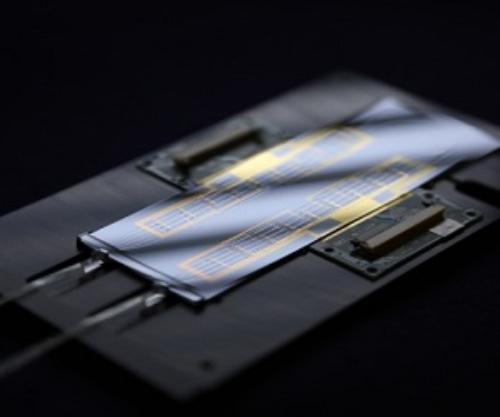
\includegraphics[width=0.5\linewidth]{1E1A7349_mod-500x417}
  \caption{\label{fig:ulo} A reprogrammable chip from [CHS+15]}
  \end{figure}
  \end{center}
  \end{itemize}
  \end{block}

  \begin{block}{\Large 3. What issues do we have?}
  \begin{itemize}
  \item Photon sources are not deterministic, so photons might not be generated at the same time.
  \item This leads to distinguishability, where photons can be identified from wavelength, time, polarisation etc.
  \item Photons might also be lost due to issues such as coupling or absorption.
  \item These cause photons to behave individually, rather than collectively.
  \end{itemize}
  \begin{center}
  \begin{figure}
  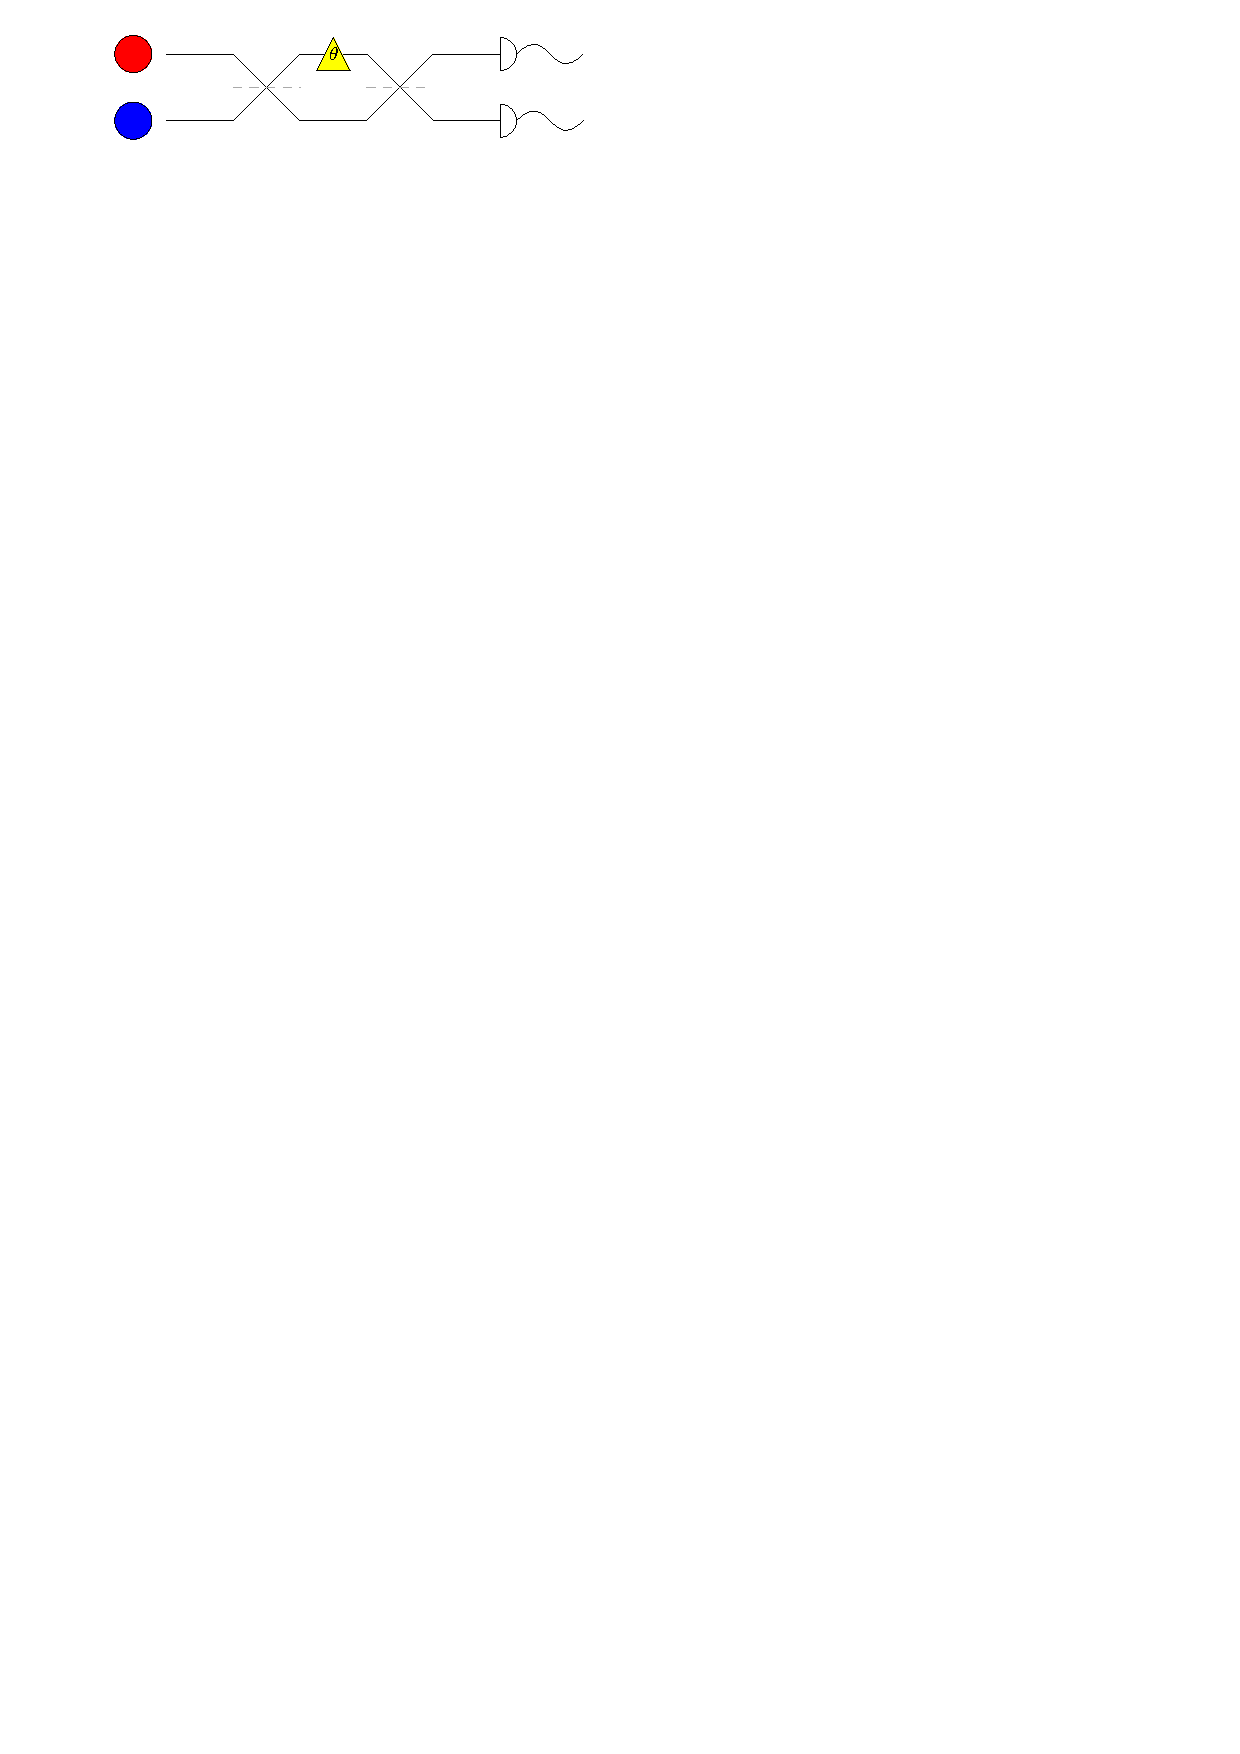
\includegraphics[width=0.45\linewidth]{dist}
  \hfill
  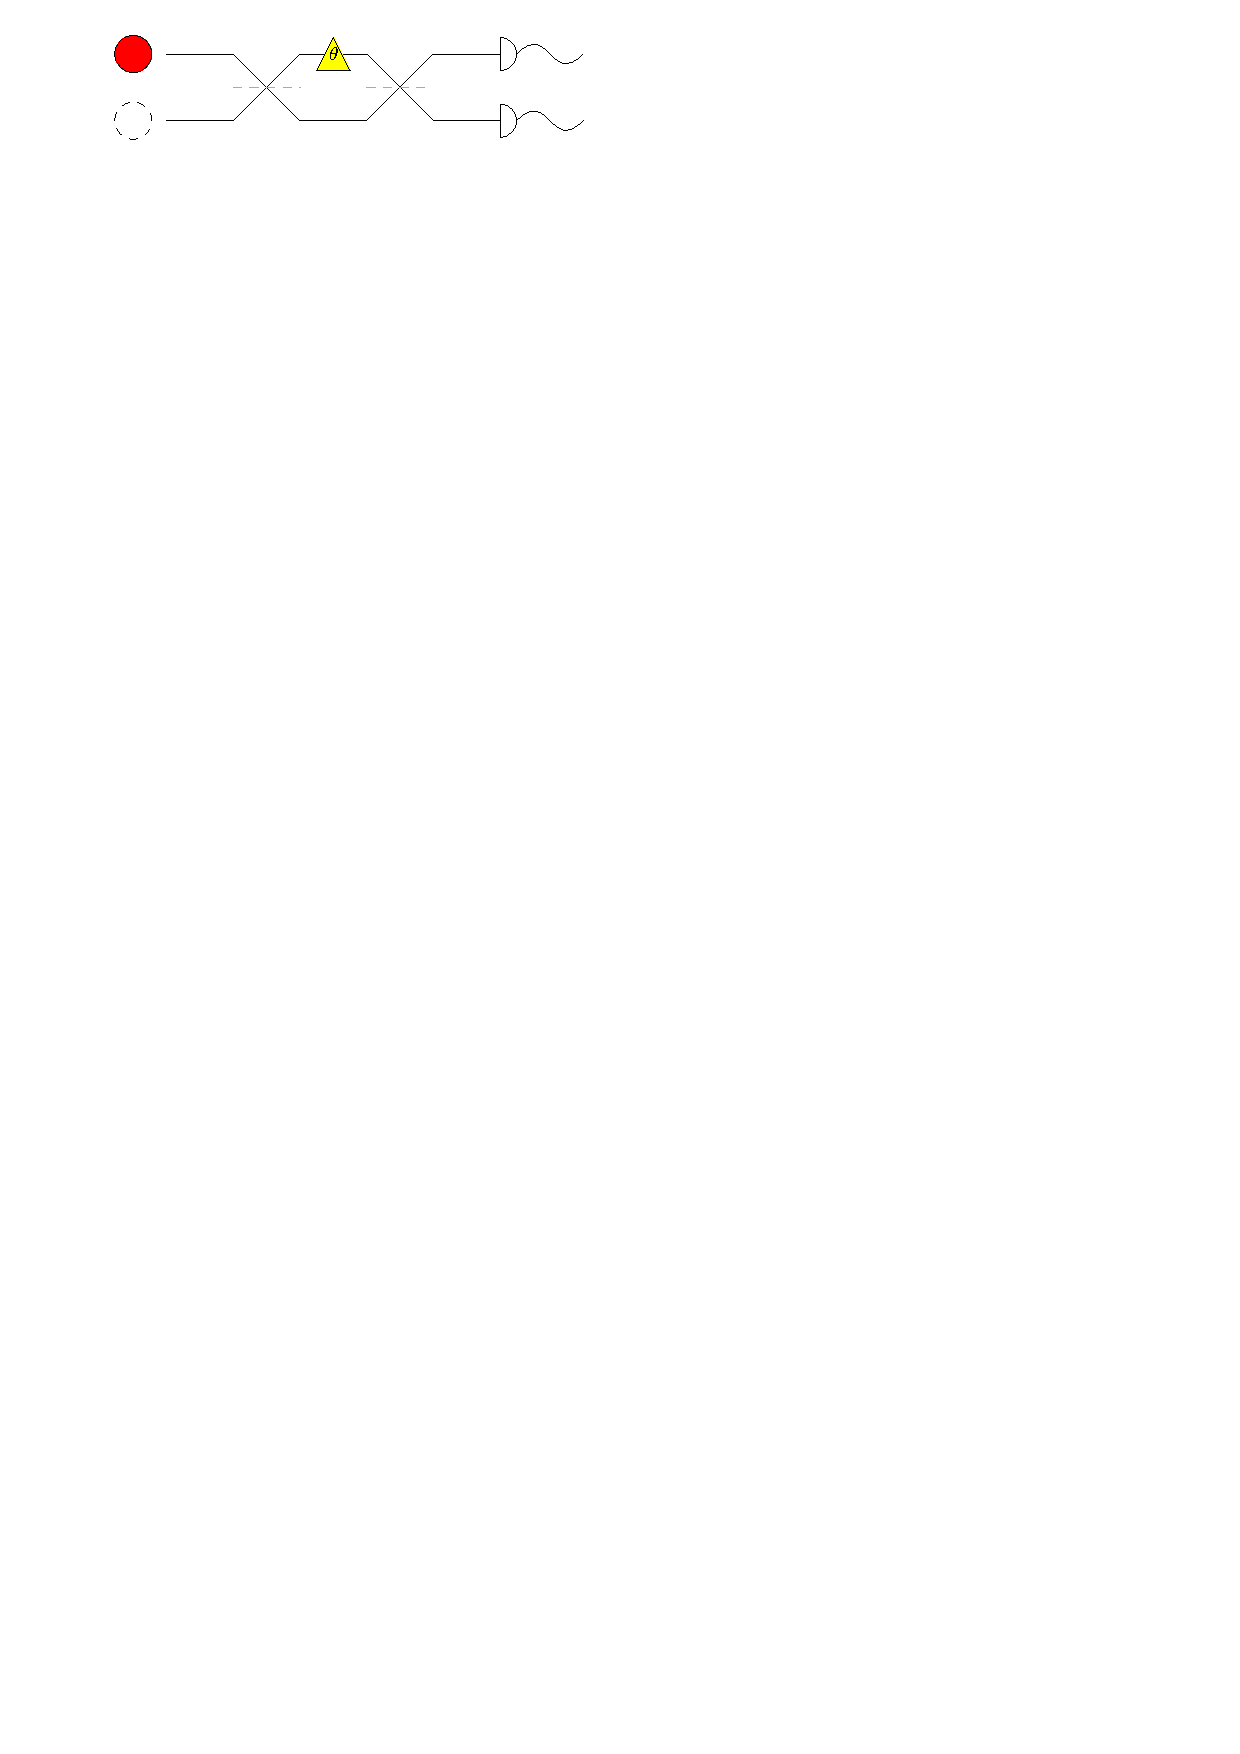
\includegraphics[width=0.45\linewidth]{loss}
  \caption{\label{fig:issues} Example issues: Distinguishability (left) and Loss (right).}
  \end{figure}
  \end{center}
  \end{block}
  \end{column}

  \begin{column}{0.422\linewidth}
  
  \begin{block}{\Large 4. A new classical simulator}
  \begin{itemize}
  \item We show that models for distinguishability $x$ [RMC+18] and loss $\eta$ [RSG-P18] are equivalent to sampling from the binomial distribution.
  \item A classical simulator for $n$-photon quantum computers:
  \begin{enumerate}
  \item Sample up to $n$ photons which survive
  \item Sample up to $k<n$ indistinguishable photons
  \item Efficiently simulate the $n-k$ distinguishable photons
  \item Simulate the $k$ indistinguishable photons in $O(k^22^k)$ time via [CC18]
  \end{enumerate}
  \end{itemize}
  \end{block}
  
  \begin{block}{\Large 5. How well does our simulator perform?}
  \begin{center}
  \begin{figure}
  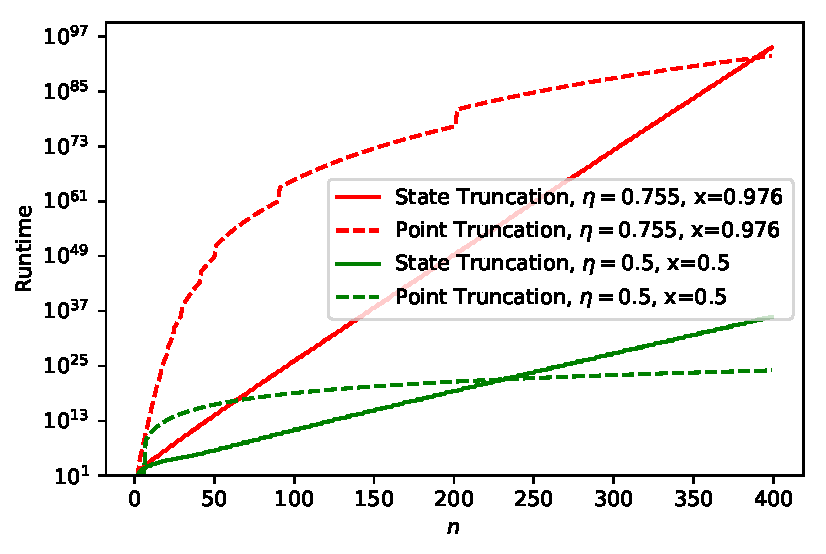
\includegraphics[width=0.45\linewidth]{runtime}
  \hfill
  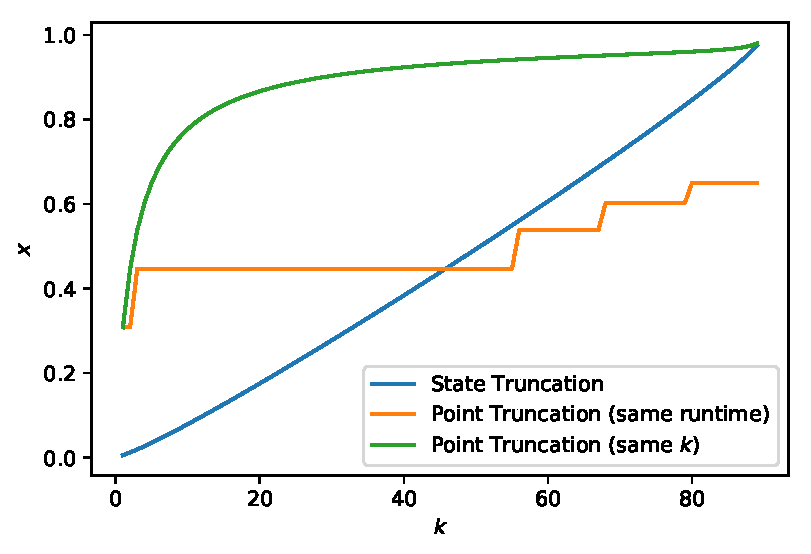
\includegraphics[width=0.45\linewidth]{max_x_fixed_n_90}
  \caption{\label{fig:performance} Estimated performance of our algorithm compared to methods of [RMC+18, RSG-P18].}
  \end{figure}
  \end{center}
  \begin{itemize}
  \item We approximate our algorithm's performance under various amounts of distinguishability ($x$) and loss ($\eta$).
  \item We demonstrate that for near-term quantum computers with 50-90 photons our algorithm can simulate more distinguishability and loss than other approaches.
  \end{itemize}
  
  \end{block}
  
  \begin{block}{\Large 6. Loss from circuit depth}
  \begin{itemize}
  \item Suppose each photon has some probability $\tau$ of surviving with every component it interacts with.
  \item Probability of photons surviving after $s$ components scales as $\tau^s$.
  \item Leads to efficient classical simulation if
  \begin{equation}
  s>\frac{\log n-\log 1/x-\log k}{\log1/\tau}.
  \end{equation}
  \item Currently all fully reprogrammable designed have at least linear depth in $n$.
  \end{itemize}
  \end{block}
  
  \begin{block}{\Large 7. Future work}
  \begin{itemize}
  \item Can we adapt classical simulation algorithms to other systems, such as quantum computers with nonlinear optics?
  \item The quantum computers considered here are non-universal. Are there ways of simulating universal quantum computers with these techniques?
  \end{itemize}
  \end{block}

  \begin{block}{\Large References}
  
  \noindent [CC+18] P. Clifford and R. Clifford, in Proc. SODA'18, 146-155 (2018)
  
  \noindent [CHS+15] J. Carolan et al., Science 349, 711-716 (2015)
  
  \noindent [IBM] IBM Quantum Experience, \url{https://quantum-computing.ibm.com/}
  
  \noindent [RMC+18] J. J. Renema et al., Phys. Rev. Lett. 120, 220502 (2018)
  
  \noindent [RSG-P18] J. J. Renema et al., [\texttt{arXiv:1809.01953}] (2018)
  \end{block}
  \end{column}
\end{columns}

\end{frame}

% -----------------------------------------------------------------------------

\end{document}